%Dave's handout 1.7 intro 2nd derivatives
%Dave's handout 2.2 2nd derivative rule
%Calaway page 143; info about 2nd derivatives
\vspace{-0.25 in}
\begin{framed}
\subsection*{Objectives}
\begin{itemize}
    \item Be able to compute the $2^{nd}$ derivative of a function using the basic rules
    \item Be able to interpret second derivatives in some real-world applications.
    \item Be able to interpret the second derivative in terms of the change in the (first) derivative or the change the slope of a curve.
    \item Be able to identify the sign of the (first) derivative the sign of the second derivative from the graph or the table of a function.
    \item Be able to determine concavity and find the inflection points from the graph of a function.
    \item Be able to determine concavity and find the inflection points given a function.
    \item Be able to determine the point of diminishing returns as an inflection point.
    \item Be able to interpret and apply the point of diminishing returns in the business context.
\end{itemize}

%%%Reading Assignment%%%
\subsection*{Suggested Reading:}
\begin{itemize}
\item \cite{Calaway}\footnotemark[1]
   \begin{itemize}
        \item \emph{Section 2.6 Second Derivative and Concavity}
    \end{itemize}

\item \cite{Hoffman}\footnotemark[2]
    \begin{itemize}
        \item \emph{Section 3.4: Second Derivative and the shape of $f$})
        \begin{itemize}
            \item Skip $f''$ \emph{and Extreme Values of} $f$.
        \end{itemize}
        
    \end{itemize}
\end{itemize}
%\subsection*{Supplemental Materials:}
%%%Key Terms%%%
\subsection*{Key Terms and Concepts:} 

\begin{multicols}{2}
\begin{itemize}
    \item $1^{st}$ derivative vs. $2^{nd}$ derivative
    \item Increasing and decreasing functions
    \item Concave up vs. Concave down
    \item Inflection points
    \item Velocity vs. Acceleration
    \item Point of Diminishing Return
\end{itemize}
\end{multicols}
\end{framed}
\footnotetext[1]{Available free to download from \url{http://www.opentextbookstore.com/details.php?id=14} .}
\footnotetext[2]{Available free to download from \url{https://www.opentextbookstore.com/details.php?id=11#tabs-3}.}
\newpage
%%%%%%%%%%START LESSON CONTENT%%%%%%%%%%%%%
%\noindent\makebox[\linewidth]{\rule{\textwidth}{0.8pt}}
\Opensolutionfile{ans}[ans7]
\Opensolutionfile{ansL}[ansL7]
%%%%%%%%%%%%%%%%Start First Topic%%%%%%%%%%%%%%%%%%%%%%%%%%%%%
\subsection*{Second Derivatives}
The derivative of a function $f$ is a function that gives information about the slope of $f$. The derivative tells us if the original function is increasing or decreasing. Because $f'$ is a function, we can take its derivative. This second derivative also gives us information about our original function $f$. The second derivative gives us a mathematical way to tell how the graph of a function is curved. \textbf{The second derivative tells us if the original function is concave up or down}.

\noindent For a given function $f(x)$, the $2^{nd}$ derivative, denoted by $f''(x)$ or $\dfrac{d^{2} y}{dx^2}$, is found by determining the derivative of $f'(x)$.  
%%Dave's 1.7--More on Derivatives; Ex1
\begin{example}
Given $f(x)=\displaystyle\frac{1}{x}+x^2$, find $f''(x)$.    %%short answer
    \begin{sol}
    $f''(x)=\displaystyle\frac{2}{x^3}+2$
    \end{sol}
    %%solution
    \begin{solL}
    Complete solution here.....
    
    \end{solL}
    
\end{example}
\vspace{0.6in}
%%Dave's 1.7--More on Derivatives; Ex2
\begin{example}
Given $f(x)=\displaystyle\frac{2}{x-3}$, find $f''(x)$. 
    \begin{sol}
    $f''(x)=\displaystyle\frac{4}{(x-3)^3}$
    \end{sol}
    %%solution
    \begin{solL}
    Complete solution here.....
    
    \end{solL}
    
\end{example}
\vspace{0.6in}
\noindent The (\emph{first}) derivative of a function $f$ is a function that gives information about the slope of f. \textbf{The (\emph{first}) derivative tells us if the original function is increasing or decreasing}.\\\\
Not all increasing (or decreasing) functions behave in the same manner. The second derivative allows us to examine in more detail how a function increases or decreases in an interval. Specifically, \textbf{the second derivative, tells us how fast the original function is increasing (or decreasing)}. See Example \ref{acceleration}.

\begin{example}\label{acceleration}
Let $s(t)=6t^3-81t^2+360t$ be the equation of the height (in feet) of a particle at time $t$ seconds. 
\renewcommand{\labelenumi}{(\alph{enumi})}
\begin{enumerate}[leftmargin=*]
    \item Find a function for the \textbf{velocity}: $v(t)=$\rule{3cm}{0.25mm}.\vspace{0.8in}
    \item Find a function for the \textbf{acceleration} of the particle: $a(t)=$\rule{3cm}{0.25mm}.\vspace{0.6in}
    
\end{enumerate}
%%short answer
    \begin{sol}
     \renewcommand{\labelenumi}{(\alph{enumi})}
     \begin{enumerate}
         \item $v(t)=18t^2-162t+360$
         \item $a(t)=36t-162$
     \end{enumerate}
    \end{sol}
%%solution
    \begin{solL}
        Complete solution here.....
    \end{solL}       
        
\end{example}


\subsection*{Concavity}

The second derivative is important when we analyze graphs of functions and the behavior of functions. It gives us a mathematical way to tell how the graph of a function is curved. \textbf{The second derivative tells us if the original function is concave up or down.}\\\\
Graphically, a function is \textbf{concave up} if its graph is curved with the \textbf{opening upward} (a in the figure). Similarly, a function is \textbf{concave down} if its graph \textbf{opens downward}. Notice that a function can be concave up regardless of whether it is increasing or decreasing.
\newpage
%%MOM QUESTION ID 266454

\begin{wrapfigure}[9]{l}{0.4\textwidth}
\begin{figure}[H]
\center
\caption{}
\label{fig:MOM266454}
\vspace{-1cm}
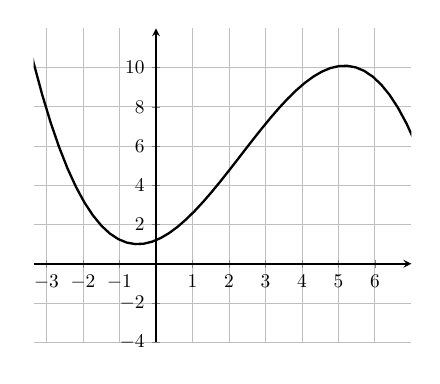
\begin{tikzpicture}[scale=0.7]
        \begin{axis}[ axis lines=middle, grid,xtick={-3,...,6},ytick={-4,-2,...,10},samples=100,ymax=12,ymin=-4,xmax=7,domain=-8:15, thick]
            \addplot+[no marks,very thick,black] {-0.1*((x+0.5)^2)*(x-8)+1 };
        \end{axis}
    \end{tikzpicture}

\end{figure}
\end{wrapfigure}
\hfill \break
\vspace{-1cm}
\begin{example}
Given the graph of a function in figure \ref{fig:MOM266454}, determine the concavity on each interval below.\\
$(-\infty,2)$:\rule{2cm}{0.25mm} \emph{(concave up/concave down)}.\\\\\\
$(2,\infty)$:\rule{2.25cm}{0.25mm} \emph{(concave up/concave down)}.\\\\

    %%short answer
    \begin{sol}
    concave up on $(-\infty,2)$; concave down on $(2,\infty)$
    \end{sol}
    %%solution
    \begin{solL}
    Complete solution here.....
    
    \end{solL}
    
\end{example}

%%% Contemporary Calculus by Hoffman; 3.4 SECOND DERIVATIVE AND THE SHAPE OF f

\begin{tcolorbox}[title = {The Second Derivative Condition for Concavity}]
\renewcommand{\labelenumi}{(\alph{enumi})}
\begin{enumerate}[leftmargin=*]
    \item If $f''(x)>0$ on an interval $I$, then $f'(x)$ is increasing on $I$ and $f$ is concave up on $I$.
    \begin{itemize}[leftmargin=*]
        \item $f'(x)$ is \emph{increasing} on $I$ means $f$ is increasing (or decreasing) \textbf{at an increasing rate}.
    \end{itemize}
    \item If $f''(x)<0$ on an interval $I$, then $f'(x)$ is decreasing on $I$ and $f$ is concave down on $I$.
    \begin{itemize}[leftmargin=*]
        \item $f'(x)$ is decreasing on $I$ means $f$ is increasing (or decreasing) \textbf{at an decreasing rate}.
    \end{itemize}
    \item If $f''(x)=0$, then $f(x)$ may be concave up or concave down or neither at $a$.
\end{enumerate}
\end{tcolorbox}


%%MOM question id 15935 (For each of four tables, identify if the table is increasing/decreasing and concave up/down)
\begin{example}
For each of four tables in table \ref{table:ConavityTable}, identify if the table is increasing/decreasing and concave up/down
\begin{table}[H]
    \begin{center}
       \begin{multicols}{4}
        \subcaptionbox{}{
        
            \begin{tabular}{|l|l|}
                \hline
                $x$ & $f(x)$\\
                \hline
                1	&	3\\
                \hline
                2	&	12\\
                \hline
                3	&	27\\
                \hline
                4	&	48\\
                \hline
                5	&	75\\
                \hline
                6	&	108\\
                \hline
            \end{tabular}
        }
       
        \subcaptionbox{}{
            \begin{tabular}{|l|l|}
                \hline
                 $x$ & $g(x)$\\
                \hline
                1	&	108\\
                \hline
                2	&	75\\
                \hline
                3	&	48\\
                \hline
                4	&	27\\
                \hline
                5	&	12\\
                \hline
                6	&	3\\
                \hline
            \end{tabular}
        }
        
        \subcaptionbox{}{
            \begin{tabular}{|l|l|}
                \hline
                $x$ & $h(x)$\\
                \hline
                1	&	92\\
                \hline
                2	&	125\\
                \hline
                3	&	152\\
                \hline
                4	&	173\\
                \hline
                5	&	188\\
                \hline
                6	&	197\\
                \hline
            \end{tabular}
        }
        
        \subcaptionbox{}{
            \begin{tabular}{|l|l|}
                \hline
                $x$ & $k(x)$\\
               \hline
                1	&	197\\
                \hline
                2	&	188\\
                \hline
                3	&	173\\
                \hline
                4	&	152\\
                \hline
                5	&	125\\
                \hline
                6	&	92\\
                \hline
            \end{tabular}
        }
 \end{multicols}   
    \caption{}
    \label{table:ConavityTable}
    \end{center}
\end{table}

    %%short answer
    
    \begin{sol}
    (a) increasing; concave up (b) decreasing; concave up (c) increasing; concave down (d) decreasing; concave down

    \end{sol}
    %%solution
    \begin{solL}
    Complete solution here.....
    \end{solL}
\end{example}
\vspace{-0.5in}
%%%Practice 1 from Hoffman; section 3.4 ; page 3
%%Problem 2 from 2.6 Exercises from Calaway
%%Table of values from MOM Question ID 15935
%%Problem 5,11 from 2.6 Exercises from Calaway
%%an inflection point occurs at f''(x)=0 but not all a such that f''(a)=0 is an inflection point
%%finding possible inflection points



%%MOM question id 2039 (Identify signs (+,-,0) of f, f ', and f '' at a point on graph of f )
\begin{wrapfigure}[7]{l}{0.4\textwidth}
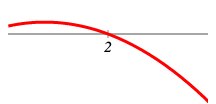
\includegraphics[width=0.8\textwidth]{2ndDervConcavity/MOM2039a.png}
\caption{ }
\label{fig:MOM2039a}
\end{wrapfigure}
\hfill \break
%\vspace{-1cm}
\begin{example}
Determine the signs (\emph{positive, negative}, or \emph{zero}) of $y=f(x)$ (shown in figure \ref{fig:MOM2039a}) and $f'(x)$ and $f''(x)$ when $x=2$.

\renewcommand{\labelenumi}{(\alph{enumi})}
    \begin{enumerate}
        \item The sign of $f(2)$ is \rule{1cm}{0.25mm}.
        \item The sign of $f'(2)$ is \rule{1cm}{0.25mm}.
        \item The sign of $f''(2)$ is \rule{1cm}{0.25mm}.
    \end{enumerate}
    %%short answer
    \begin{sol}
    \renewcommand{\labelenumi}{(\alph{enumi})}
    \begin{enumerate}
        \item zero
        \item negative
        \item negative
    \end{enumerate}
    \end{sol}
    %%solution
    \begin{solL}
    Complete solution here.....
    
    \end{solL}
    
\end{example}
\vspace{0.6in}

%%%Examples%%%
%%%question 5 from Handout 5.2 from MATH 142 spring 2019 by Maya Johnson at Texas A&M university; handout download from
%%%handout can be downloaded from https://www.math.tamu.edu/~mayaj/m142_Chapter5_Sec5.2completed.pdf
\begin{example}
Given the following statements, answer the questions below.
\begin{tcolorbox}[colback=white,boxrule=0.15mm]
Let $x=a$ be on an interval $I$.
\begin{multicols}{2}
\begin{enumerate}[leftmargin=*]
    \item $h''(a)>0$ ($h''(a)$ is positive.)
     \item $h''(a)<0$ ($h''(a)$ is negative.)
    \item $h'(a)>0$ ($h'(a)$ is positive.)
    \item $h'(a)<0$ ($h'(a)$ is negative.)
    \item $h'(a)$ is increasing.
    \item $h'(a)$ is decreasing.
    \item The slope of a line tangent to the graph of $h$ is decreasing on an interval $I$.
    \item The slope of a line tangent to the graph of $h$ is increasing on an interval $I$ .
    \item The slope of a line tangent to the graph of $h$ at $x=a$ is positive.
    \item The slope of a line tangent to the graph of $h$ at $x=a$ is negative.
\end{enumerate}
\end{multicols}
\end{tcolorbox}


\renewcommand{\labelenumi}{(\alph{enumi})}
\begin{enumerate}
    \item Which of the statements given above are equivalent to the statement that $h(x)$ is \textbf{increasing} at $x=a$? Choose all that apply.
    \item Which of the statements given above are equivalent to the statement that $h(x)$ is \textbf{decreasing} at $x=a$? Choose all that apply.
    \item Which of the statements given above are equivalent to the statement that $h(x)$ is \textbf{concave up} on an interval $I$? Choose all that apply.
    \item Which of the statements given above are equivalent to the statement that $h(x)$ is \textbf{concave down} on an interval $I$? Choose all that apply.
\end{enumerate}

    %%short answer
    \begin{sol}
    (a) 3,9 (b) 4,10 (c) 1,5,8 (d) 2,6,7
    \end{sol}
    %%solution
    \begin{solL}
    Complete solution here.....
    
    \end{solL}
    
\end{example}

%%%Epidemic Examples from Applied Calculus; section 2.6 Calaway%%%
\begin{wrapfigure}[17]{l}{0.4\textwidth}
\vspace{-.5cm}
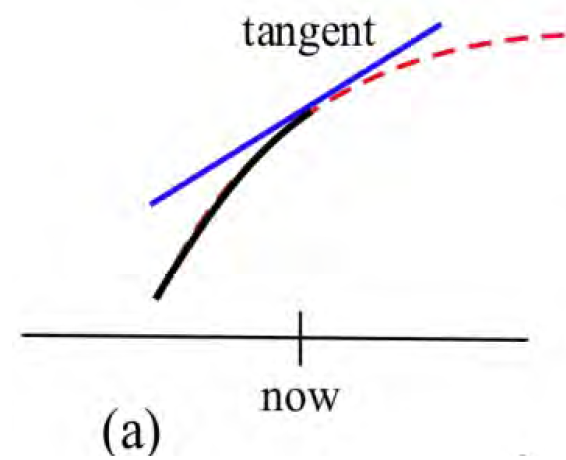
\includegraphics[width=0.6\textwidth]{2ndDervConcavity/epidemicA.png}
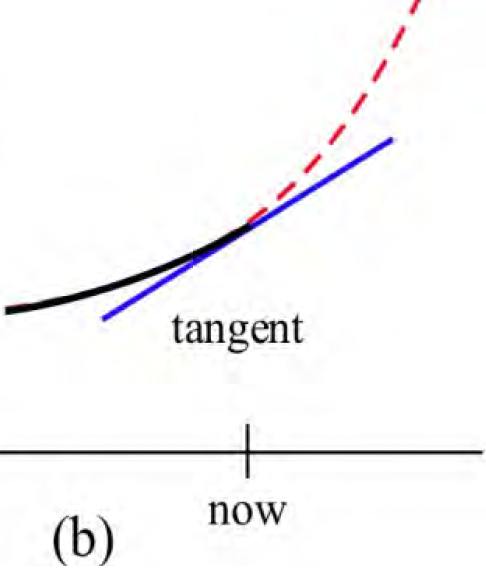
\includegraphics[width=0.5\textwidth]{2ndDervConcavity/epidemicB.png}
\caption{ }
\label{fig:epidemic}
\end{wrapfigure}

\hfill \break
\vspace{-1.25cm}
\begin{example}{\label{epidemic}}
\textbf{An Epidemic:} Suppose an epidemic has started, and you, as a member of congress, must decide whether the current methods are effectively fighting the spread of the disease or whether more drastic measures and more money are needed. In the figure \ref{fig:epidemic}, $f(x)$ is the number of people who have the disease at time $x$, and two different situations are shown. In both (a) and (b), the number of people with the disease, $f(now)$, and the rate at which new people are getting sick, $f '(now)$, are the same. The difference in the two situations is the concavity of $f$, and that difference in concavity might have a big effect on your decision.\\

\noindent In (a), $f$ is concave \rule{2cm}{0.25mm}(\emph{up or down}) at "now", the slopes are \rule{4cm}{0.25mm}\\(\emph{increasing or decreasing}), and it looks as if it’s tailing off. We can say "$f$ is increasing at a \rule{2cm}{0.25mm}\emph{(increasing rate or decreasing rate)}". Does it appear that the current methods are starting to bring the epidemic under control? \rule{2cm}{0.25mm}(\emph{Yes or No})\\
\hfill \break
\noiindent In (b), $f$ is concave \rule{2cm}{0.25mm}(\emph{up or down}) at "now", the slopes are \rule{4cm}{0.25mm}\\(\emph{increasing or decreasing}). We can say "$f$ is increasing at a \rule{2cm}{0.25mm}\emph{(increasing rate or decreasing rate)}". Does it appear that the current methods are starting to bring the epidemic under control? \rule{2cm}{0.25mm}(\emph{Yes or No})
    %%short answer
    \begin{sol}
    (a) down;decreasing;decreasing rate;yes. (b) up;increasing;increasing rate;no.
    \end{sol}
    %%solution
    \begin{solL}
    Complete solution here.....
    
    \end{solL}
    
\end{example}
\vspace{0.6in}
%%%%%%%%%%%%%%%%%%%%%%%%%%%%%%%%%%%%%%%%%%%%%%%%%%%%%%%%
\subsection*{Inflection Points}
\begin{tcolorbox}[title={Definition}]
An \textbf{inflection point} is a point on the graph at which the function is \emph{continuous} and the concavity of the graph changes from concave up to down or from concave down to up.
\end{tcolorbox}

%%%Examples%%%
%%Example 4 from 2.6 Calaway
\begin{example}
Let $f(x)=x^3$, $g(x)=x^4$ and $h(x)=x^{1/3}$ For which of these functions is the point (0,0) an inflection point? Use figure \ref{fig:inflection1} and fill in table \ref{table:inflection1} to help you answer the question.
\begin{figure}[h]
    \centering
    \caption{} 
    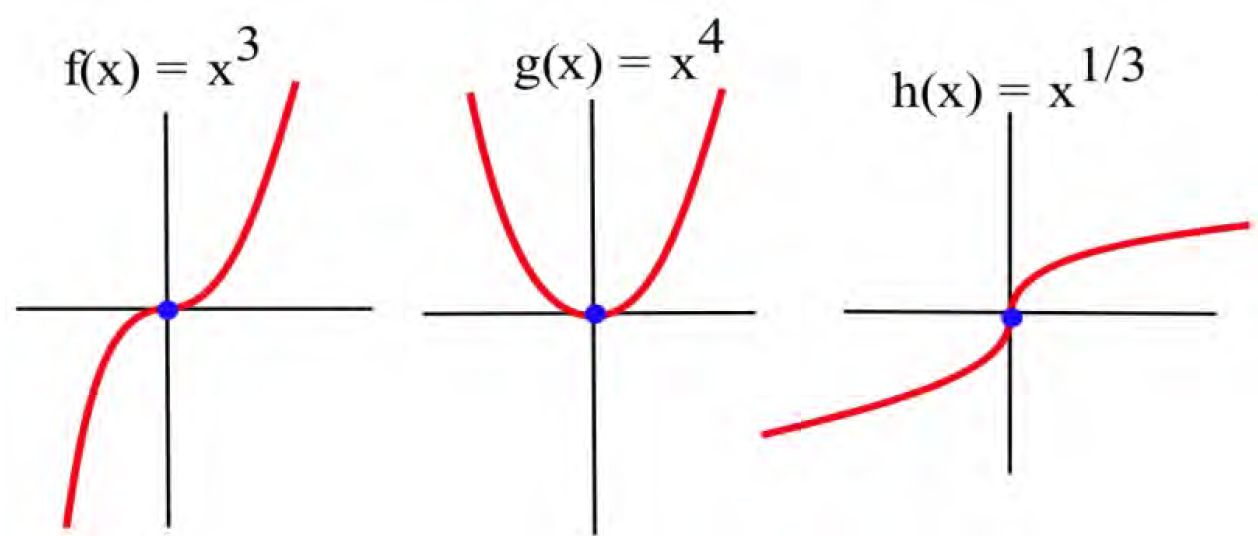
\includegraphics[scale=0.5]{images/2ndDervConcavity/inflection1.png} 
    \label{fig:inflection1}
\end{figure}
%%%%%%%%%%%%%%%%%%%%%%%%%%%%%%%%%%%%%%%
\begin{table}[h]
\centering
\begin{tabular}{ | m{5cm} | m{2cm}| m{2cm} | m{2cm}|} 
\hline
 &$f(x)=x^3$&$f(x)=x^4$& $f(x)=x^{1/3}$\\
\hline
Concave up/down on $(-\infty,0)$ & & & \\
\hline
Concave up/down on $(0,\infty)$ & & & \\ 
\hline
Change in concavity (yes/no) & & & \\ 
\hline
Inflection point (yes/no) & & & \\ 
\hline
\end{tabular}
\caption{}
\label{table:inflection1}
\end{table}
%%%%%%%%%%%%%%%%%%%%%%%%%%%%%%%%%%%%%%%%
    %%short answer
    \begin{sol}
    yes;no;yes
    \end{sol}
    %%solution
    \begin{solL}
    Complete solution here.....
    
    \end{solL}
    
\end{example}

%%%Examples%%%
%%Example 3 from 2.6 Calaway
\begin{example}
Which of the labeled points in the graph below are inflection points?
\begin{figure}[h]
    \centering
    \caption{} 
    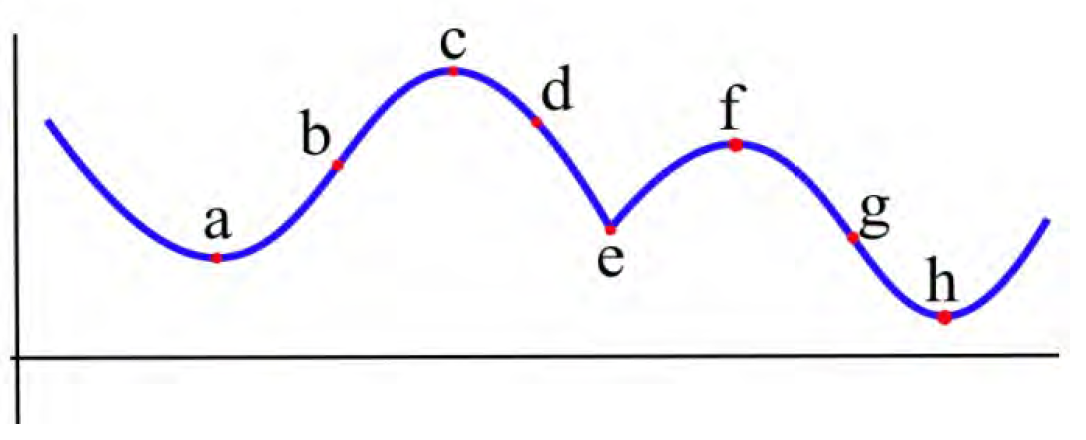
\includegraphics[scale=0.6]{images/2ndDervConcavity/inflection2.png} 
    \label{fig:inflection1}
\end{figure}
    %%short answer
    \begin{sol}
    b and g
    \end{sol}
    %%solution
    \begin{solL}
    Complete solution here.....
    
    \end{solL}
    
\end{example}
\vspace{0.6in}
%MATH 142 spring 2019 by Maya Johnson at Texas A&M university; handout download from https://www.math.tamu.edu/~roquesol/Math142_Spring_2011_Lecture_5.2.pdf
\begin{tcolorbox}[title={Concavity Test: Determine Concavity and Inflection Values}]
\begin{enumerate}
    \item Find the values $x=c$ where $f''(c)=0$ or $f"(c)$ does not exist.
    \item Place these values of a number line and use the second derivative to generate a sign chart.
    \item The point $(c,f(c))$ is an inflection point if $f''(x)$ changes sign at $x=c$ and if $x=c$ is in the domain of $f(x)$.
\end{enumerate}
\end{tcolorbox}
%%%Examples%%%
%%%Practice 4 from Hoffman; section 3.4 
\begin{example}
Consider $f(x)=x^4-12x^3+30x^2+5x-7$. Give the intervals where $f(x)$ is concave up or down and find the x-values of any inflection points. \emph{Check your answer with the graph of $f$ on a graphing calculator.}\footnotemark
    %%short answer
    \begin{sol}
    concave up on $(-\infty,1)$; concave down on $(1,5)$; concave up on $(5,\infty)$
    \end{sol}
    %%solution
    \begin{solL}
    Complete solution here.....
    
    \end{solL}
    
\end{example}
\vspace{3in}
%%%%%%%%%%%%%%%%%%%%%%%%
%%%Examples%%%
%%%Dave's handout 2.1 
\begin{example}
Consider $f(x)=\displaystyle\frac{1}{x-1}$.Give the intervals where $f(x)$ is concave up or down and find the x-values of any inflection points. \emph{Check your answer with the graph of $f$ on a graphing calculator}.\footnotemark[\value{footnote}]
    %%short answer
    \begin{sol}
    concave down on $(-\infty,1)$; concave up on $(1,\infty)$; no inflection point.
    \end{sol}
    %%solution
    \begin{solL}
    Complete solution here.....
    
    \end{solL}
    
\end{example}
\vspace*{\fill}
\noindent \emph{Result: The concavity of a graph may change at a value of x for which the function is not defined (not in the domain).  As such, this is not considered an inflection point. }
\footnotetext{Access Desmos Graphing Calcuator from \url{https://www.desmos.com/calculator}. Access Geogebra Graphing Calculator from \url{https://www.geogebra.org/graphing}. You may find the following tutorial videos helpful for basic graphing in Desmos: \url{https://youtu.be/7oVOs9TX57s} and \url{https://youtu.be/En_PkyA-4_4} }
%%%Additional Examples%%%
%%%questions 5-7 from Handout 5.2 from MATH 142 spring 2019 by Maya Johnson at Texas A&M university; handout download from
%%%handout can be downloaded from https://www.math.tamu.edu/~mayaj/m142_Chapter5_Sec5.2completed.pdf

%%%%%%%%%%%%End Examples%%%%%%%%%%%%%%%%%%
%%%%%%%%%%%%%%%End Topic%%%%%%%%%%%%%%%%%%
%%%%%%%%%%%%%%%%Begin Next Topic%%%%%%%%%%%%%%%%%%%%%%%%%%%%%%%

\subsection*{Applications of Second Derivative}
%%%%%%%%%%%%End Examples%%%%%%%%%%%%%%%%%%
%%%%%%%%%%%%%%%End Topic%%%%%%%%%%%%%%%%%%
\begin{tcolorbox}[title={Law of Diminishing Returns\footnotemark[1]}]
In economics the \textbf{law of diminishing returns} says that anytime you increase one factor of production (e.g.  employees, machinery, fertilizer, etc) while keeping all other factors of production constant, eventually you will hit a \textbf{point of diminishing returns},where the incremental per-unit returns begin to drop.
\end{tcolorbox}
\footnotetext[1]{https://math.mit.edu/seminars/esme/misc/2017-11-21_Gerhardt_Business-Lab.pdf}
%%%%Source: http://www.evlm.stuba.sk/~velichova/xmathkluc/diff/practise/applic/app15.xml
\begin{example}
A company estimates that it will have the revenue R(x) from sales after spending $x$ on advertising their product, as given by
\begin{center}
    $R(x)=\displaystyle\frac{1}{10000}(300x^2-x^3)$,\hspace{10pt} $0\le x\le 200$
\end{center}
where the revenue $R(x)$ and the advertising cost $x$ are both measured in million of Euros.\\
Given the graph of $R(x)$ shown in figure \ref{fig:diminishR1} , answer the following questions.
\begin{figure}[h]
    \centering
    \caption{} 
    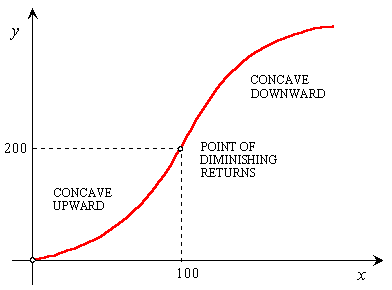
\includegraphics[scale=0.5]{images/2ndDervConcavity/diminishR1.png} 
    \label{fig:diminishR1}
\end{figure}
\renewcommand{\labelenumi}{(\alph{enumi})}
\begin{enumerate}[leftmargin=*]
    \item Using the \emph{Concavity Test}, show that the \textbf{point of diminishing returns} is the inflection point of $R$.
   \newpage
    \item \textbf{Fill in the blanks:} In the interval $(0,100)$, each additional Euro invested in advertising increases sale \rule{2cm}{0.25mm} (\emph{more or less}) than the previous Euro invested in advertising. The is because the slope of the curve is \rule{2cm}{0.25mm} (\emph{increasing or decreasing}) on $(0,100)$.\vfill
    \item \textbf{Fill in the blanks:} In the interval $(100,200)$, the slope of the curve is \rule{2cm}{0.25mm} (\emph{increasing or decreasing}) and each additional Euro invested in advertising increases sale \rule{2cm}{0.25mm} (\emph{more or less}) than the previous Euro invested in advertising.\vfill
    \item If the company currently put 100 millions of Euros in advertising, would you recommend the company to invest more on the advertising? Why or why not?\vfill
\end{enumerate}
%%short answer
    \begin{sol}
    (a) concave up on $(-\infty,100)$; concave down on $(100,\infty)$; Change in concavity at $x=100$ $\Longrightarrow$ inflection point at $x=100$. (b) more;increasing (c) decreasing;less (d) no.
    \end{sol}
    %%solution
    \begin{solL}
    Complete solution here.....
    
    \end{solL}
\end{example}

\newpage

\begin{figure}[H]
    \centering
    \caption{} 
    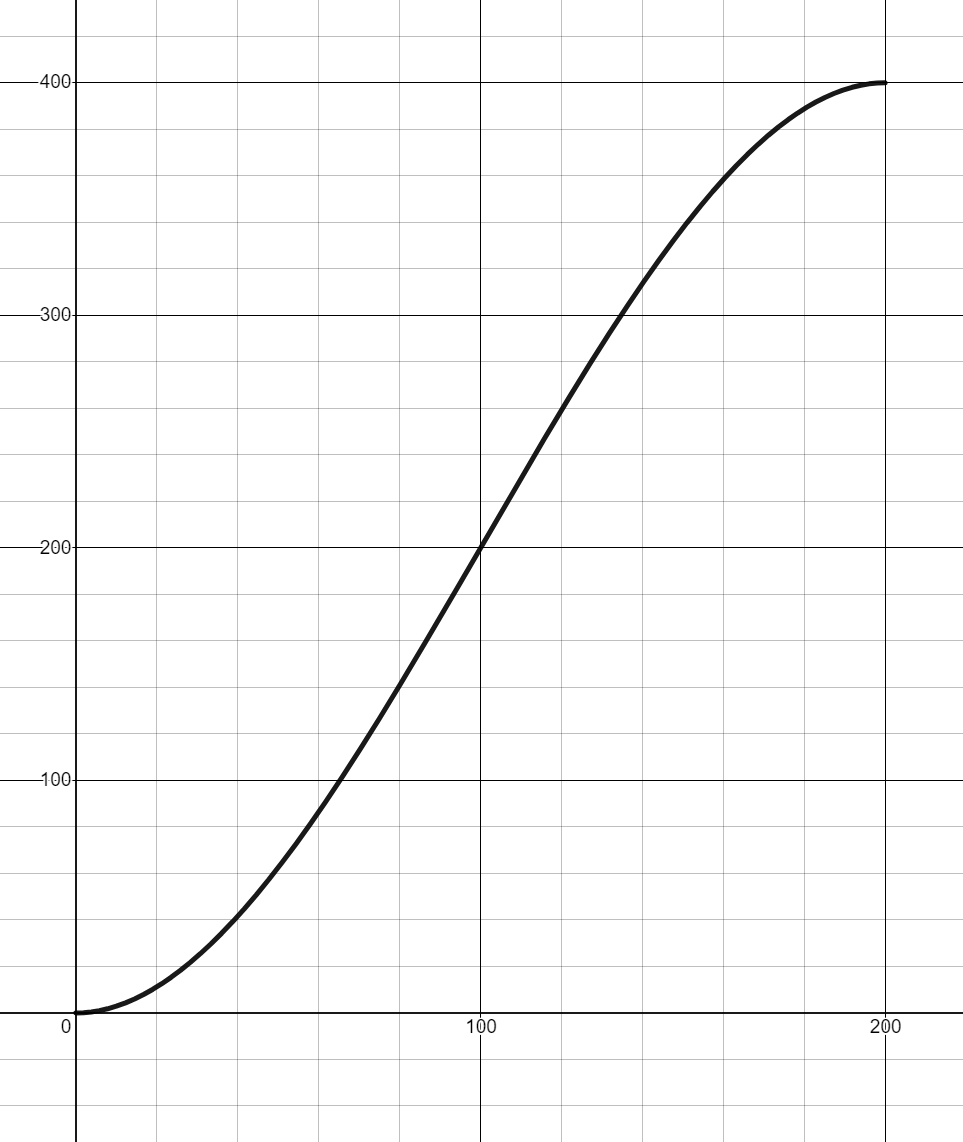
\includegraphics[scale=0.75]{images/2ndDervConcavity/diminishingReturn_ex1_graph2.PNG} 

\end{figure}


\begin{figure}[H]
    \centering
    \caption{} 
    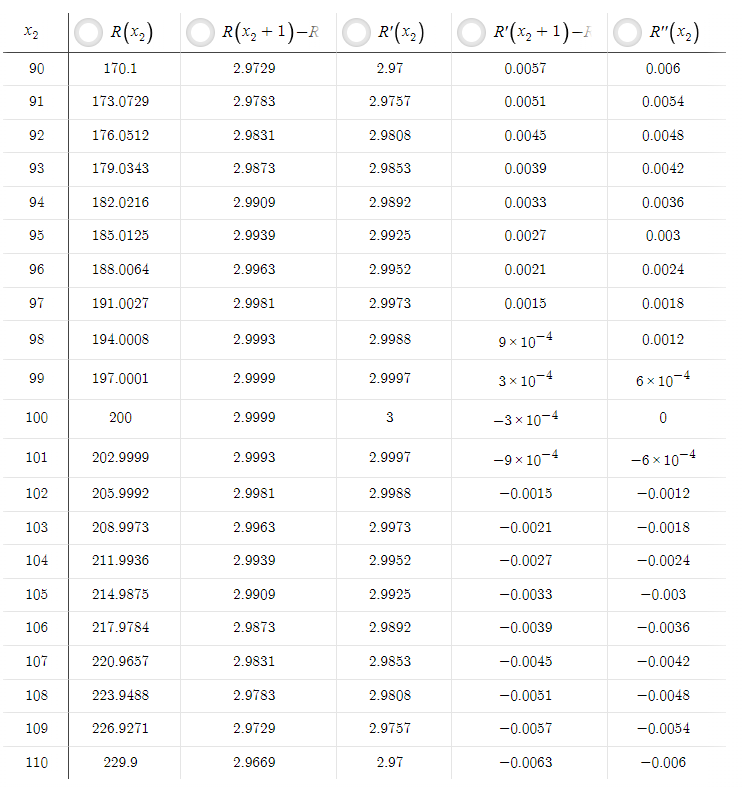
\includegraphics[scale=1.9]{images/2ndDervConcavity/diminishingReturn_ex1_table2.PNG} 

\end{figure}
\footnotetext[1]{
Source: \url{https://www.desmos.com/calculator/fi82bbco2v}}
\newpage
\subsection*{Second Derivative Test for Extremes}
\noindent The concavity of a function can also help us determine whether a critical point is a maximum or minimum or neither. For example, if a point is at the bottom of a concave up function, then the point is a minimum (see figure \ref{fig:oneLocalExtrema}). 
\begin{tcolorbox}[title={The Second Derivative Test for Extremes:}]
\begin{enumerate}[leftmargin=*]
    \item Find the \textbf{domain} of $f$.
    \item Find all \textbf{critical numbers} of $f$.
    \item For those critical points where $f'(c)=0$, find $f''(c)$.
    \item Locate any \textbf{local extrema} by determining the sign of $f''(c)$ as follows:
    \renewcommand{\labelenumi}{(\alph{enumi})}
    \begin{enumerate}[leftmargin=*]
        \item If $f''(c)<0$ then $f$ is \textbf{concave down} and has a \textbf{local maximum} at $x=c$.
        \item If $f''(c)>0$ then $f$ is \textbf{concave up} and has a \textbf{local minimum} at $x=c$.
        \item If $f''(c)=0$ then $f$ may have a local maximum, a minimum or neither at $x=c$.
    \end{enumerate}
\end{enumerate}
\end{tcolorbox}
\vspace{-0.25cm}
\begin{example}
\noindent Given $f(x)=x+\displaystyle\frac{100}{x-1}$, determine all \textbf{local extrema} by using the \emph{Second Derivative Test for Extremes} as described above. You may use the \emph{critical numbers} of $f$ that were already found in part c of Example \ref{1stDervTestLocal_ex7}. Compare your results to the results from using \emph{First Derivative Test for Extremes} in the example. 
%%short answer
    \begin{sol}
    local max at $x=-9$; local min at $x=11$; same results.
    \end{sol}
    %%solution
    \begin{solL}
    Complete solution here.....
    
    \end{solL}
\end{example}


%%%%%%%%%%%%%%%End Lesson%%%%%%%%%%%%%%%%%%
\Closesolutionfile{ans}
\Closesolutionfile{ansL}

%%%Short Answers to Examples%%%
\newpage
%\vspace*{\fill}
\subsection*{Short Answers to Examples}
%\vspace{-0.25cm}
\begin{multicols}{2}
\input{ans7}
\end{multicols}


